\chapter{Kết quả và đánh giá}
\label{chapter4}
Sau khi đã xây dựng thành công thuật toán đã trình bày trong 3, em tiến hành thực nghiệm để phát hiện và điều chỉnh để thuật toán đa truy nhập tốt hơn. Chương này, em xin trình bày về những kết quả đã đạt được và hướng phát triển của đề tài.
\section{Các kết quả đạt được}
\subsection{Phân tích kết quả các thử nghiệm}
Sau khi tự động cấu hình, nó sẽ gửi yêu cầu tham gia mạng đến Gateway và bắt đầu gửi tin (nếu được Gateway chấp thuận). Hình \ref{receivePacket} mô tả quá trình kiểm tra yêu cầu tham gia mạng của nút và nhận gói tin từ nút.
\begin{figure}[h]
\centering
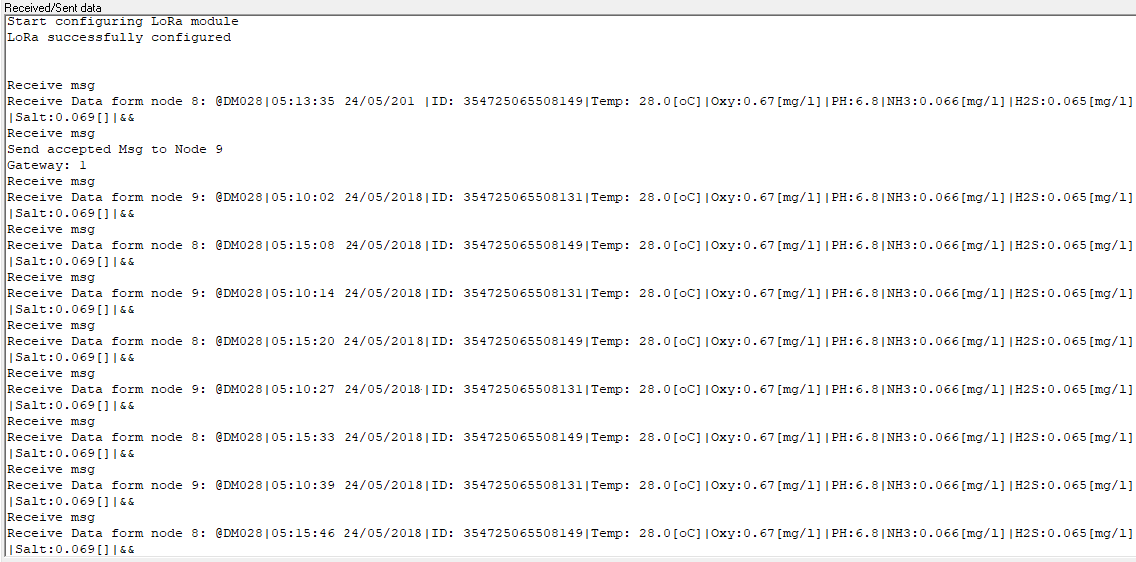
\includegraphics[scale=0.4]{image/receivePacket}
\caption{Quá trình xử lý của Gateway}
\label{receivePacket}
\end{figure}
\subsubsection{Thử nghiệm 1: Đánh giá mất gói trong điều kiện thuận lợi (PTN)}
Thử nghiệm này được triển khai tại phòng nghiên cứu Sanslab, thí nghiệm thực hiện gồm có 3 nút và 1 gateway. Các thông số kỹ thuật được cấu hình như trong Bảng \ref{bang3_1}, các nút nằm trong bán kính 10 m của Gateway. Ngoài ra có hai số thông số được thiết lập trước là ID của nút và ID của Gateway. Kết quả của thực nghiệm được mô tả trong Bảng \ref{TN1} và biểu đồ Hình \ref{sendrate}{}.\\
\begin{table}[h]
\centering
\caption{Bảng kết quả độ mất gói trong điều kiện thuận lợi}
\label{TN1}
\begin{tabular}{|c|c|c|c|}
\hline
 & Nút 2 & Nút 3 & Nút 4 \\
 \hline
 Gửi gói tin thành công & 98,77,02 \% & 98,98 \% & 100 \% \\
 \hline
 Hủy gói tin & 1,23 \% & 1,03 \% & 0 \% \\
 \hline
\end{tabular}
\end{table}
\begin{figure}
\centering
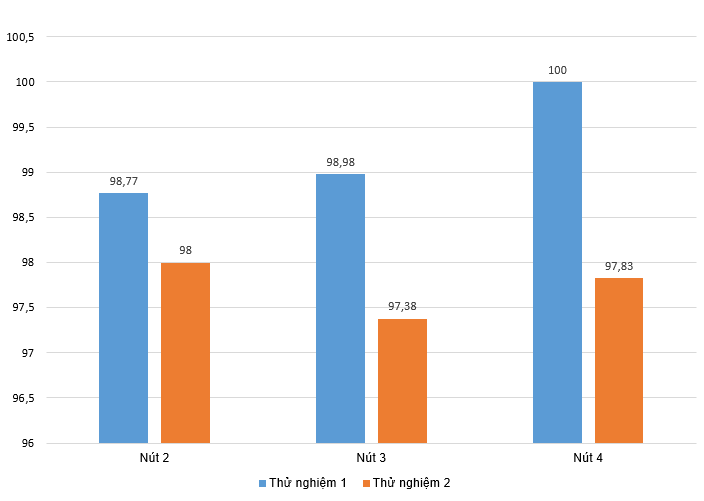
\includegraphics[scale=0.5]{image/sendrate}
\caption{Kết quả thí nghiệm đánh giá độ mất gói}
\label{sendrate}
\end{figure}
\subsubsection{Thử nghiệm 2: Đánh giá độ mất gói trong điều kiện thách thức}
Thử nghiệm 2 được thực hiện tại khuôn viên Đại học Bách Khoa Hà Nội, các thông số kỹ thuật của thử nghiệm 2 được thiết lập giống với thử nghiệm 1. Trong thử nghiệm này, Gateway được đặt tại tầng 6 thư viện Tạ Quang Bửu, nút đặt rải rác trong khuôn viên trường với môi trường có vật cản. Kết quả thử nghiệm 2 được ghi lại trong Bảng \ref{TN2} và được biểu diễn trên Hình \ref{sendrate}{}.\\
\begin{table}[h]
\centering
\caption{Bảng quả độ mất gói trong điều kiện thách thức}
\label{TN2}
\begin{tabular}{|c|c|c|c|}
\hline
 & Nút 2 & Nút 3 & Nút 4 \\
 \hline
 Gửi bản tin thành công & 98,0 \% & 97,38 \% & 97,83 \% \\
 \hline
 Hủy bản tin & 2,0 \% & 2,62 \% & 2,17 \% \\
 \hline
\end{tabular}
\end{table}
\subsubsection{Đánh giá kết quả thử nghiệm}
Trong cả 2 thử nghiệm, độ mất gói là rất nhỏ (nhỏ hơn 3\%) chứng tỏ thuật toán đa truy nhập hoạt động tốt với số lượng nút nhỏ (3 nút). Bên cạnh đó, tỷ lệ mất gói của thử nghiệm 2 cao hơn thử nghiệm 1, cho thấy được khoảng cách và vật cản có ảnh hưởng đến độ mất gói trong quá trình truyền dữ liệu.
\subsection{Hệ thống BKRES-LoRa}
Công nghệ LoRa đã được phòng nghiên cứu Sanslab áp dụng vào hệ thống BKRES thành công. Module truyền thông được tích hợp vào kit điều khiển (hình \ref{KitBKRES_LoRa}{}) với kích thước gọn nhẹ, tiêu tốn ít năng lượng (module sử dụng Pin để cung cấp năng lượng).
\par 
Những bản tin Gateway nhận được sẽ được gửi đến server và những dữ liệu đó được hiển thị các ứng dụng (hình \ref{Webapp}{}).\\
\begin{figure}[h]
\centering
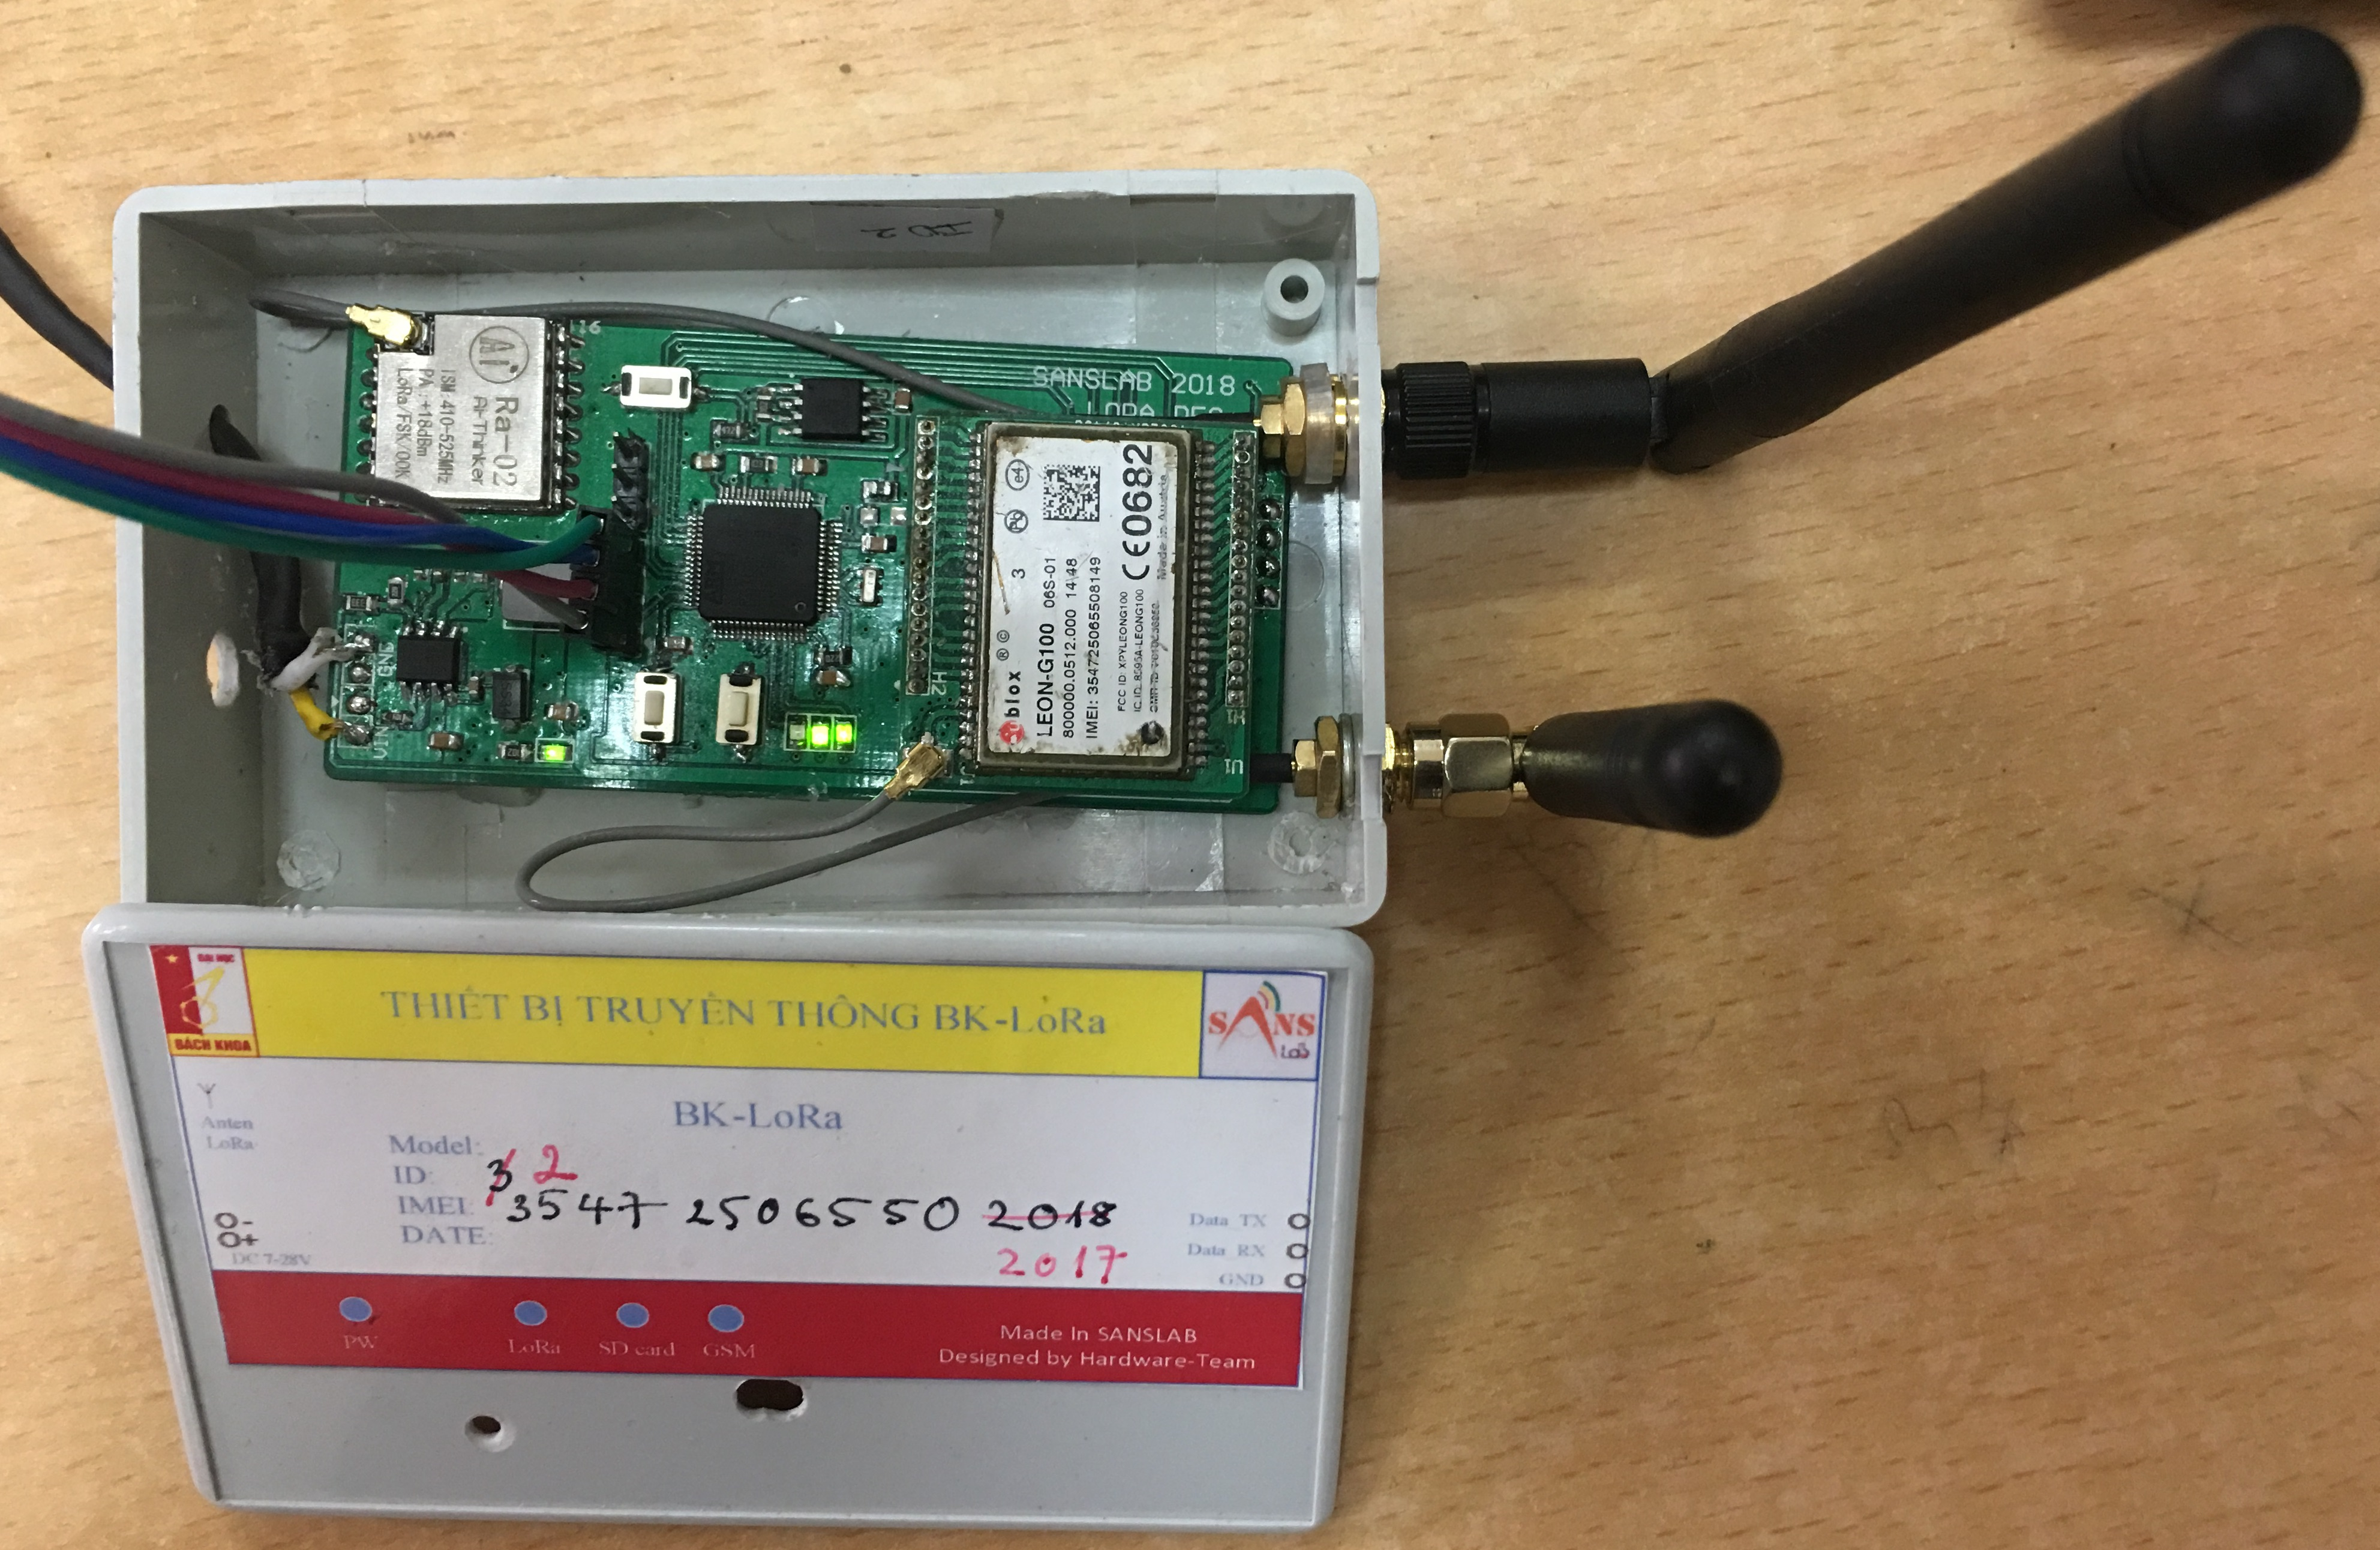
\includegraphics[scale=0.08]{image/KitBKRES_LoRa}
\caption{Kit điều khiển BKRES-LoRa}
\label{KitBKRES_LoRa}
\end{figure}\\
\begin{figure}[h]
\centering
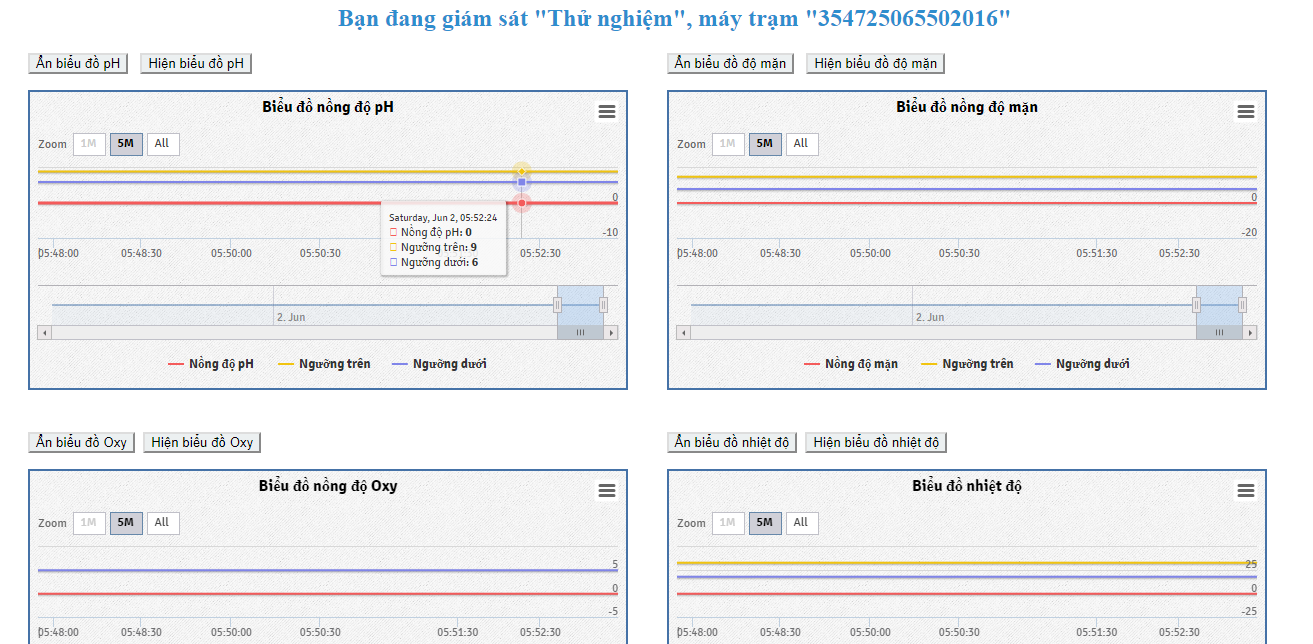
\includegraphics[scale=0.3]{image/application}
\caption{Hiển thị dữ liệu trên ứng dụng web}
\label{Webapp}
\end{figure}
\section{Đánh giá thuật toán và định hướng phát triển}
Thuật toán đa truy nhập có những ưu điểm và nhược điểm sau:
\begin{itemize}
\item Ưu điểm:
	\begin{itemize}
	\item	Thuật toán hoạt động tốt,
	\item	Hiệu năng truyền gói thành công cao hơn nhiều so với các giao thức truy nhập ngẫu nhiên khác,
	\item	Các thiết bị sử dụng thuật toán hoạt động ổn định, tiêu thụ ít năng lượng (so với sử dụng module sim).
	\end{itemize}
\item Nhược điểm:
	\begin{itemize}
	\item 	Chưa xác định được độ ảnh hưởng của số lượng thiết bị đến thuật toán,
	\item	Chưa xác định được các thời gian tiêu tốn để thực hiện các quá trình (tham gia mạng, gửi dữ liệu) để điều chỉnh trễ hợp lý,
	\item	Quá trình yêu cầu tham gia mạng phức tạp, ảnh hưởng đến quá trình gửi tin của nút khác,
	\item	Năng lượng tiêu thụ của Gateway lớn (vì Gateway không có khoảng thời gian để nghỉ),
	\item 	Hầu như chưa có sự quản lý của Gateway đối với các nút trong mạng.
	\end{itemize}
\end{itemize}
\par 
Thuật toán cần được phát triển hơn nữa để có thể tăng hiệu năng, độ ổn định của những thiết bị trong mạng và áp dụng cho mạng có số lượng nút lớn. Ngoài ra để tăng khoảng cách truyền, cần phát triển giao thức áp dụng cho mô hình mạng đa chặng để giảm số lượng Gateway trong mạng.
\section{Kết luận}
Qua kết quả của những thử nghiệm đã được tiến hành, chứng tỏ thuật toán đa truy nhập hoạt động tốt với số lượng nút nhỏ (3 nút), do điều kiện về số lượng thiết bị giới hạn nên em chưa xác định được kết quả hoạt động của thuật toán đa truy nhập trong mạng có số lượng nút lớn hơn. Ngoài ra, thuật toán đa truy nhập đã được thích hợp vào hệ thống BKRES-LoRa thành công.